\documentclass[11pt]{article}
\usepackage[T1]{fontenc}
\usepackage[utf8]{inputenc}
\usepackage{lmodern}
\usepackage[a4paper,margin=29mm,headheight=15pt]{geometry}
\usepackage{amsmath,amssymb,amsthm,mathtools}
\usepackage{microtype,booktabs,array,enumitem}
\usepackage[dvipsnames]{xcolor}
\usepackage{tikz}
\usetikzlibrary{arrows.meta,positioning,calc,fit,backgrounds}
\usepackage{fancyhdr}
\definecolor{ink}{HTML}{16364B}
\definecolor{accent}{HTML}{A34D3B}
\definecolor{soft}{HTML}{EDF2F4}
\usepackage[colorlinks=true,linkcolor=ink,citecolor=ink,urlcolor=ink,
 pdfauthor={Petri Mikael Autio},
 pdftitle={Determinate Preservation: Hegelian Sublation and the Homotopy of Resolving Levels}]{hyperref}
\usepackage[nameinlink,noabbrev]{cleveref}
\hypersetup{pdfsubject={Philosophy of mathematics; Hegel; Aufhebung; truncated homotopy types; Kan extensions}}
\pagestyle{fancy}
\fancyhf{}
\fancyhead[L]{\small\textsc{Determinate preservation}}
\fancyhead[R]{\small Petri Mikael Autio}
\fancyfoot[C]{\small\thepage}
\renewcommand{\headrulewidth}{0.3pt}
\setlength{\parindent}{1.2em}
\setlength{\parskip}{0.15em}
\setlist{nosep,topsep=5pt}
\emergencystretch=1.5em
\numberwithin{equation}{section}
\theoremstyle{plain}
\newtheorem{theorem}{Theorem}[section]
\newtheorem{proposition}[theorem]{Proposition}
\newtheorem{lemma}[theorem]{Lemma}
\newtheorem{corollary}[theorem]{Corollary}
\theoremstyle{definition}
\newtheorem{definition}[theorem]{Definition}
\newtheorem{example}[theorem]{Example}
\theoremstyle{remark}
\newtheorem{remark}[theorem]{Remark}
\newcommand{\Set}{\mathbf{Set}}
\newcommand{\Spc}{\mathcal S}
\newcommand{\Vk}{\mathcal V_k}
\newcommand{\Fun}{\operatorname{Fun}}
\newcommand{\Map}{\operatorname{Map}}
\newcommand{\Lan}{\operatorname{Lan}}
\newcommand{\Ran}{\operatorname{Ran}}
\newcommand{\res}{\operatorname{res}}
\newcommand{\sk}{\operatorname{sk}}
\newcommand{\cosk}{\operatorname{cosk}}
\newcommand{\colim}{\operatorname*{colim}}
\newcommand{\hocolim}{\operatorname*{hocolim}}
\newcommand{\limop}{\operatorname*{lim}}
\newcommand{\B}{\mathrm B}
\newcommand{\N}{\mathrm N}
\newcommand{\Z}{\mathbb Z}
\newcommand{\Aup}{\mathsf A}
\newcommand{\Ccat}{\mathcal C}
\newcommand{\Pcat}{\mathcal P}
\newcommand{\K}{\mathrm K}
\newcommand{\tr}{\tau_{\leq k}}
\begin{document}
\hypersetup{pageanchor=false}
\begin{titlepage}
\vspace*{17mm}
{\color{accent}\large\textsc{Philosophy \& mathematics}}\par
\vspace{9mm}
{\color{ink}\Huge\bfseries Determinate Preservation\par}
\vspace{5mm}
{\LARGE Hegelian Sublation and the Homotopy\par of Resolving Levels\par}
\vspace{12mm}
{\Large Petri Mikael Autio\par}
\vspace{3mm}
{22 October 2026\par}
\vspace{12mm}
\begin{abstract}
Lawvere's categorical rendering of Hegelian sublation makes preservation
precise through least resolving levels. We study two choices on which
such leastness depends: the relations represented and the coefficient
semantics governing generation and reconstruction.
For diagrams over a finite poset, a matching-map argument gives the least
full reconstruction subset for any specified diagram family, and hence
for arbitrary starting levels. For constant generation this becomes an
upper-interval criterion. We compute coefficient-relative resolution
profiles from sets through truncated homotopy types. A Boolean family
has explicit wedge-of-sphere obstructions and arbitrarily many distinct
least levels, although every earlier resolution comparison remains
unchanged. A compact family realizes $m$ distinct levels on $2m+2$
objects; for an initial one-object level, the first set-to-groupoid jump
requires exactly six. The jump
also survives nonconstant generation. Without preservation of generation,
a second family reverses the inclusion: richer coefficients require fewer
positions. A further comparison, grounded in
an interactive reader of the \emph{Science of Logic}, orders the same
positions by ancestry or succession. Both profiles are invariant under
coefficient enrichment, yet their least subsets differ sharply.
Together these calculations show why old-test agreement does not secure
later leastness, and why coefficient stability does not establish an
interpretation. Reading these results alongside Hegel's accounts of
retention, mediation, and method, we defend determinate preservation:
a reconstruction must make its asserted mode of retention and its
interpretive warrant answerable together. The resulting comparison with
nLab and contemporary formalizations separates mathematical necessity
within a representation from justification of the relations and tests
that produce it.
\end{abstract}
\vfill
{\small\color{ink}Keywords: Hegel; Science of Logic; Aufhebung; categorical logic;
Kan extension; truncated spaces; philosophy of formalization.\par}
\vspace{3mm}
{\small Research manuscript. Mathematical proofs and reproducible finite checks
are included; this version has not undergone external peer review.\par}
\end{titlepage}
\hypersetup{pageanchor=true}
\pagenumbering{roman}
\begingroup\footnotesize\setlength{\parskip}{0pt}
\tableofcontents
\endgroup
\newpage
\pagenumbering{arabic}
\section{The question hidden inside preservation}
\label{sec:intro}

A mathematical reconstruction of Hegelian sublation makes two
commitments: it selects relations that represent the content, and it
selects tests under which that content counts as preserved. Universal
properties can determine a result once those commitments are fixed.
They do not by themselves establish that the commitments express the
intended mediation. We investigate this distinction through exact
calculations of least resolving levels. The calculations show both how
an expanded test domain can change a least result while preserving every
earlier comparison, and how stability across test domains can leave the
interpretation of the represented relations unsettled.

For the first comparison, the relevant enrichment replaces
sets by homotopy types. A set distinguishes its elements; a homotopy type also
allows identifications between elements, identifications between those
identifications, and further coherent structure. The issue is therefore not
merely whether the same symbols remain available in a more elaborate
foundation. The universal constructions denoted by those symbols can change.
A compatibility condition that is sufficient for sets can leave a detectable
obstruction when paths and higher paths are admitted.

The philosophical importance of the question comes from sublation. In the
\emph{Science of Logic}, Hegel distinguishes the result of mediation from an
empty disappearance. In the remark on the expression \emph{Aufheben}, the
earlier determination persists in a changed status: its immediacy is cancelled,
but it is not simply annihilated \cite{HegelSublation}. Whatever else one takes
this to mean, a mathematical reconstruction should explain which aspect of the
earlier determination remains available and in what sense. The bare word
``preservation'' does not yet provide that explanation.

Lawvere's theory supplies a demanding candidate. A level has both a skeletal
and a sheaf presentation in an ambient topos. A higher level resolves it when
the earlier skeleta become sheaves at the higher level. An Aufhebung is a
\emph{least} resolving level. This is substantially stronger than enclosing two
objects in a third. The construction has a mathematical order, an explicit
factorization condition, and a minimality claim
\cite{KennettEtAl,Menni}. The question we ask is whether such leastness is
unchanged when the coefficients become homotopical.

Our answer is negative in a controlled and quantitative sense. We keep the
finite indexing poset and the initial level fixed. We change only the category
of coefficients, from sets to groupoids and then to successively higher
truncated spaces. Every earlier resolution comparison remains unchanged,
including the construction of the objects being tested. Nevertheless the
least resolving full-subcategory level changes at every stage until the whole
indexing category is required. Agreement on every earlier test does not
therefore secure stability of the least adequate reconstruction. This is the
stronger claim we defend, beyond a general reminder that models have
parameters.

\subsection{The result in advance}

For $N\geq3$, let $\Pcat_N$ be the poset of nonempty proper subsets of
$[N]=\{1,\ldots,N\}$. Place two objects $b<a$ below every element of
$\Pcat_N$, obtaining a poset $\Ccat_N$ with $2^N$ objects. The starting level
is $D=\{b\}$. We work with covariant functor categories, equivalently with
presheaves on the opposite posets. Because $b$ is initial, extension from $D$
produces constant diagrams.

For $k\geq0$, let $\Vk=\Spc_{\leq k}$ be the category of $k$-truncated
spaces. Thus $\mathcal V_0\simeq\Set$, while $\mathcal V_1$ may be presented
by groupoids. A full subposet $R$ containing $b$ resolves $D$ if every constant
$\Vk$-valued diagram on $\Ccat_N$ is a right Kan extension of its restriction
to $R$. The main theorem computes the least such $R$:
\begin{equation}\label{eq:introformula}
\Aup_k(D)=
\begin{cases}
\{b\}\,\cup\,\{S\in\Pcat_N:|S|\geq N-k-2\},&0\leq k\leq N-3,\\
\Ccat_N,&k\geq N-2.
\end{cases}
\end{equation}
For unrestricted spaces the answer is also $\Ccat_N$. The word ``least''
here refers to \emph{all} full subposets containing $b$, not merely to a
preselected chain of rank cuts. The restricted class of levels is explicit;
we do not assume a classification of all higher essential subtoposes.

The proof identifies the comparison map at an object $x$ with
\[
A\longrightarrow\Map\bigl(\B(x\downarrow R),A\bigr).
\]
For a proposed resolver, the omitted information is therefore encoded by a
comma-category nerve. At $a$, the nerve for the first line of
\eqref{eq:introformula} is a wedge of
$\binom{N-1}{k+2}$ spheres of dimension $k+1$. These spheres are invisible
to $k$-types but visible to $(k+1)$-types. The theorem is consequently more
informative than an isolated failure of transfer: it specifies how much
coherence each resolution leaves untested.

\subsection{What is and is not claimed as a contribution}

The topology of simplex skeleta, the formula for a limit of a constant
space-valued diagram, and the relation between truncation and connectivity are
standard. They are proved or recalled below and are not proposed as new
foundational results. The contribution offered here is a worked theory of finite
coefficient-relative resolution profiles: a matching-support formula,
explicit leastness calculations, a linear-size family with a sharp
six-object first jump, a nonconstant extension, and a reverse family
in which changed generation makes the least resolver smaller. The formula is an
elementary consequence of Reedy reconstruction, not a new foundation for
it. The philosophical argument pairs the changed-test calculation with
a reader-based comparison in which coefficient stability fails to settle
the interpretation of relations. These comparisons give distinct,
precise tasks to the requirement of determinate preservation.

The finite calculations have a methodological use. The paper
does not solve the general problem of transporting Aufhebung between arbitrary
topoi. It does not derive the sequence of Hegel's categories, and it does not
identify the sphere in an example with a contradiction in Hegel's text. Its
claim is that the family supplies a counterexample to a tempting methodological
inference: mathematical leastness in one semantic setting does not, by itself,
establish leastness in a richer one.

The relevant background is wider than the vocabulary of Aufhebung.
Truncated cofinality already explains why higher coefficients require more
coherent limit data \cite{Du}. We use that background rather than claiming to
rediscover it. What remains to be assessed by further specialist comparison is
whether the specific finite resolution family has appeared in another form.
The argument for its philosophical significance does not depend on presenting
its elementary ingredients as previously unknown.

The ordinary finite-poset endpoint also meets recent work on minimal initial
functors. Dey and Lesnick describe a least full subposet sufficient for
ordinary limit computation, as well as finer minimality questions allowing
relations to be removed \cite{DeyLesnick}. Our coefficient-indexed profile
should be compared with that work and with truncated cofinality, not
presented as a new general theory of ordinary minimal limit computation.

\section{Hegel, Lawvere, and the burden of a formal reconstruction}
\label{sec:philosophy}

\subsection{Three requirements that should not be collapsed}

The Introduction to the \emph{Science of Logic} connects determinate negation
with a result that has a specific content because of what it negates. Its
advance is not the replacement of one empty designation by another. The
method is also not supposed to be an independently supplied device applied
to an indifferent subject matter \cite{HegelIntro}. These commitments motivate
three distinct questions for a reconstruction.

First, there is a question of \emph{retention}. What survives the transition?
An embedding may preserve objects while changing the morphisms between them.
A quotient may preserve connected components while erasing loops. A logical
translation may preserve provable sentences while adding new inferential
relations. None of these is preservation without qualification. A reconstruction
must say which of these achievements, or which other achievement, is relevant
to the passage under interpretation.

Second, there is a question of \emph{determination}. Why is this result the
result of this earlier content? A construction that can be attached equally
well to any pair of terms may be mathematically legitimate but explanatorily
weak. What matters is not merely that something later can accommodate
something earlier. The earlier structure should contribute to specifying the
later one.

Third, there is a question of \emph{necessity}. What excludes alternatives?
A universal property can answer this question after the ambient category,
admissible constructions, and relevant equivalences have been fixed. Whether
those choices express the philosophical content is an additional question.
Confusing the two questions turns the uniqueness of an answer to a specified
problem into an argument that the problem was specified in the only adequate
way.

These requirements do not amount to a definition of Hegel's method. They
are obligations incurred by a mathematical interpretation that claims to
represent its preservation, determination, or necessity. The distinction is
important. An interpretation can meet one obligation and fail another; it can
also be mathematically productive while making only a modest claim about
Hegel.

\subsection{Why the categorical proposal deserves a serious test}

Lawvere's use of adjoint structures gives the philosophical vocabulary
mathematical consequences. His account of unity and identity of opposites
studies common retractions and their adjoint forms in examples from calculus
and physics \cite{Lawvere1996}. The value of this approach lies in the
possibility of asking whether the proposed relation exists, how it behaves,
and which further structures it entails. The resulting mathematics can resist
an interpretation as well as illustrate it.

For full subcategories of an indexing category, restriction has left and right
Kan extension adjoints. These two extensions produce different presentations
of the same smaller diagram category inside the larger one. A resolving level
requires the presentation supplied on one side of the earlier adjunction to
be accessible through the other side of the later one. Leastness then
constrains how much additional structure is admitted. In this respect,
Lawvere's formulation directly addresses determination: the earlier skeletal
image constrains which levels can count as resolutions.

The formulation also makes a hidden choice visible. A Kan extension is
computed in a category of coefficients. In sets its limits enforce ordinary
compatibility. In spaces the same notation requests coherent compatibility.
The latter includes data that the former cannot detect. The notation can
remain unchanged while the mathematical demand becomes stronger. Our
calculation makes this dependence explicit.

\subsection{A textual benchmark: from becoming to determinate being}

The transition at the beginning of the \emph{Logic} provides a demanding
benchmark. In the account of coming-to-be and ceasing-to-be, each moment's
direction passes into the other. Becoming depends on their distinction,
yet that distinction is itself unstable; its result is not an empty
return to nothing \cite{HegelBecoming}. The subsequent remark makes
retention more specific: the earlier determinations become moments whose
significance is established within their new unity \cite{HegelSublation}.

Two requirements follow for an interpretation of this particular passage.
It must explain how the earlier content supplies a reason for its
transformation, and how the retained determinations acquire their changed
significance. Merely putting copies of two objects into a third would meet
neither requirement. Exact recovery of an earlier object would meet a
retention condition, but would still not explain its changed status or
the need for the transition.

Our model leaves those two requirements open. Its indexing relations
are supplied in advance, and admitting the next coefficient category is
a decision in the construction. The theorem then forces a different least
resolver. It establishes the conditional necessity of a repair, not the
self-generated necessity of Hegel's transition. The test separates a
recoverability achievement from the stronger interpretive claims that
could otherwise be attached to it.

Hegel's Introduction itself warns against importing mathematical method
into philosophy \cite[online paragraph 62]{HegelIntro}. Our use of
mathematics is diagnostic: it examines a proposed formal correlate. It
does not claim that a calculation generates the movement of the
\emph{Logic}. This addresses the warning without pretending to settle
Hegel's wider assessment of mathematics.

\subsection{The nLab project and its stated restrictions}

nLab's \emph{Science of Logic} entry develops a modal and type-theoretic
reconstruction: concepts are treated as types, moments through modalities,
and opposition through adjoint structures. It connects an abstract treatment
with universes and categorical models. It also places restrictions on its own
results, distinguishing a 0-type argument about determinate negation from
stable-type constructions \cite{nLabLogic}. The separate Aufhebung entry
states a least resolving-level condition \cite{nLabAufhebung}.

These restrictions are examples of the discipline advocated here, not
errors that our finite example corrects. Likewise, nLab's claim that
adjoints are determined is expressly conditional on a concrete interpreted
moment. The question is how to extend comparable explicitness to the
coefficient dependence of least resolving levels. Pr\"ahauser's exposition
distinguishes a broader resolving relation from a unique least
resolution \cite{Praehauser}; terminology alone cannot supply minimality.

The present test is therefore internal to a mathematical possibility the
project itself takes seriously: movement between categorical and homotopical
settings. It is not an objection that a reconstruction fails to preserve every
distinction in every conceivable foundation. Rather, when a reconstruction
uses both ordinary and higher versions of its structures, their agreement
must be established where it is invoked. A restricted theorem remains
restricted even if its notation resembles a more general theorem.

There is a constructive way to respond. One can retain the ordinary
interpretation and justify its restriction to sets. One can strengthen the
higher reconstruction and supply the extra coherence it requires. Or one can
treat the sequence of coefficient categories as a family of distinct
interpretations with distinct explanatory purposes. Each response is more
informative than assuming that a familiar universal property carries its
philosophical force unchanged across the passage.

\subsection{Formalization as a source of philosophical questions}

One might ask whether all this is merely a technical qualification on an
analogy. It would be, if the claim under examination were only that adjunctions
resemble some aspects of opposition. The stakes change when the claim is that
a canonical or necessary transition has been exhibited. At that point,
the conditions of canonicity become part of the philosophical argument.

Hegel's discussion of determinate being offers a useful restraint here. He
distinguishes determinations present in the concept under development from
those supplied by the interpreter's comparison \cite{HegelDasein}. A
homotopical reconstruction need not deny that distinction. It should apply it
to itself. A path, a higher identity, or an ambient infinity-topos is initially
a resource of the reconstruction. Its relevance to the interpreted content
requires an argument. The mathematical theorem can sharpen that argument
by showing exactly what depends on the resource, but cannot supply the
historical or philosophical identification on its own.

\section{Coefficient-relative resolution}
\label{sec:setup}

All indexing categories in the main construction are finite ordinary posets,
regarded as categories. Their nerves are also used as indexing
infinity-categories when the coefficients are spaces. Write $\B J=|\N J|$
for the classifying space of an ordinary category $J$, with
$\B\varnothing=\varnothing$.

\subsection{Conventions and Kan extensions}

For $k\geq0$ put $\Vk=\Spc_{\leq k}$, and put
$\mathcal V_\infty=\Spc$. These categories admit the limits and colimits
used below. Limits of $k$-types agree with their limits in spaces; colimits
are obtained by taking the colimit in spaces and then truncating. When
groupoids represent 1-types, their limits here are homotopy-coherent
limits, not strict limits in the ordinary category of groupoids. We use
\emph{covariant} diagrams $\Fun(C,\Vk)$. This is the presheaf convention
on $C^{\mathrm{op}}$, not on $C$.

For a full inclusion $u:R\hookrightarrow C$, let $u^*$ be restriction. Its
adjoints are
\begin{equation}\label{eq:triple}
u_!=\Lan_u\ \dashv\ u^*\ \dashv\ u_*=\Ran_u.
\end{equation}
Both extension functors are fully faithful. On the ambient diagram category
define
\[
\sk_R=u_!u^*,\qquad \cosk_R=u_*u^*.
\]
The counit $\sk_R X\to X$ detects $R$-skeletal objects; the unit
$X\to\cosk_R X$ detects $R$-coskeletal objects. If $D\subseteq R$, the
skeletal and coskeletal presentations for $D$ factor through those for $R$,
by composition of Kan extensions. This is the ordering of the induced levels
used throughout the paper.

\begin{definition}\label{def:resolution}
Let $D\subseteq R\subseteq C$ be full subcategories. The level $R$
\emph{$k$-resolves $D$} if for every $A:D\to\Vk$ the canonical unit
\begin{equation}\label{eq:resolution}
\Lan_D A\longrightarrow \Ran_R\res_R\Lan_D A
\end{equation}
is an equivalence. A \emph{coefficient-relative Aufhebung}, written
$\Aup_k(D)$, is a least such full subcategory under inclusion, if it exists.
The definition for $k=\infty$ uses unrestricted spaces.
\end{definition}

The qualifier records a substantive restriction. For $k=0$, this is the
usual skeletal-to-coskeletal resolution condition on the specified ordinary
presheaf levels. For higher $k$, we extend the condition through
\eqref{eq:triple}. We do not silently identify the admissible family of
induced levels with every possible essential localization of a higher
category of diagrams.

\subsection{Matching maps and least reconstruction subsets}
\label{sec:matching}

The existence of a least full resolver over a finite poset can be
separated from the calculation of that resolver. Let $\mathcal V$ be an
infinity-category with finite limits. For $X:C\to\mathcal V$, write
\begin{equation}\label{eq:matchingsupport}
M_xX=\limop_{y\in C_{>x}}X(y),\qquad
S(X)=\{x\in C:X(x)\longrightarrow M_xX\text{ is not an equivalence}\}.
\end{equation}
The map is induced by the arrows out of $x$; at a maximal element its
target is terminal. These are matching objects for the inverse Reedy
structure obtained by assigning smaller degree to higher objects of
$C$. Matching objects and inductive extension of diagrams are standard
Reedy machinery \cite[section 3]{RiehlVerity}. The following elementary
consequence is useful because it applies to arbitrary full subposets,
not just degree cuts.

\begin{proposition}[Least reconstruction subset]\label{prop:support}
Let $C$ be a finite poset, $R\subseteq C$ full, and
$X:C\to\mathcal V$. The canonical unit
$X\to\Ran_R(X|_R)$ is an equivalence if and only if $S(X)\subseteq R$.
Consequently, for any specified family $\mathcal F$ of such diagrams,
the least full subposet from which every member is right Kan extended is
\begin{equation}\label{eq:familysupport}
S(\mathcal F)=\bigcup_{X\in\mathcal F}S(X).
\end{equation}
\end{proposition}

\begin{proof}
If $X$ is right Kan extended from $R$ and $x\notin R$, factor the
inclusion through $C\setminus\{x\}$. Composition of right Kan
extensions shows that $X$ is also right Kan extended from this
intermediate subposet. Its unit at the only omitted object is exactly
$X(x)\to M_xX$, because
$(x\downarrow(C\setminus\{x\}))=C_{>x}$. Thus $x\notin S(X)$.

Conversely, suppose $S(X)\subseteq R$. List the objects of
$C\setminus R$ in an increasing linear extension, and delete them in
that order. When $x$ is deleted, every $y>x$ is still present. The
comparison for right extension from the remaining subposet is an
equivalence at every retained object, and at $x$ it is the original
matching map $X(x)\to M_xX$. This is an equivalence by assumption.
Compose the finitely many right Kan extensions to obtain the assertion
for $R$. Applying the equivalence to every $X\in\mathcal F$ proves
the formula for a family.
\end{proof}

\begin{corollary}[Arbitrary starting levels]\label{cor:arbitraryD}
If $D\subseteq C$ is any full subposet and $\mathcal V$ also admits
the left Kan extensions in question, the least full resolver of $D$
exists and is
\begin{equation}\label{eq:arbitraryD}
D\,\cup\!\bigcup_{A\in\Fun(D,\mathcal V)}S(\Lan_D A).
\end{equation}
In particular this holds for every $\mathcal V_k$ used here.
\end{corollary}

This is an existence result, not a general algorithm: the quantifier
over $A$ can be substantial. It also locates the role of leastness in
our finite setting. Once a diagram family and its matching tests are
fixed, the least subset is already forced; the substantive problem is
to compute it and to justify the chosen family. No new general theory
of Reedy matching objects is claimed.

\begin{example}[Why the finiteness hypothesis matters]\label{ex:infinite}
Take $C=\mathbb N$ with its usual order and $D=\{0\}$.
Every strict upper interval has a least element, so the matching support
of every constant diagram is empty. Nevertheless a full $R$ containing
$0$ resolves constants exactly when it is unbounded: then each
$(n\downarrow R)$ has a least element, while for bounded $R$ an upper
comma is eventually empty. There is no inclusion-minimal unbounded
subset containing $0$, because any positive member may be deleted.
Thus the finite matching-support conclusion cannot be extended to
arbitrary infinite posets merely by using the same formula.
\end{example}

\subsection{Resolution of an initial one-object level}

Let $C$ have an initial object $b$, and let $D=\{b\}$. Since the comma
category $(D\downarrow x)$ has one object and its identity for every $x$,
left extension from $D$ is the constant diagram:
\begin{equation}\label{eq:constantlan}
\Lan_D A\simeq\Delta_C A.
\end{equation}
This holds for every coefficient category under consideration, including
arbitrary spaces. There is no homotopy-colimit defect in the left extension
of this particular starting level.

\begin{lemma}[Constant-diagram criterion]\label{lem:criterion}
Let $R\subseteq C$ be full and contain $b$. For finite $k\geq0$, the
following are equivalent:
\begin{enumerate}[label=(\roman*)]
\item $R$ $k$-resolves $D$;
\item $\tau_{\leq k}\B(x\downarrow R)\simeq *$ for every $x\in C$.
\end{enumerate}
For $k=\infty$, replace (ii) by contractibility of every
$\B(x\downarrow R)$.
\end{lemma}

\begin{proof}
Pointwise right Kan extension and \eqref{eq:constantlan} identify the
comparison at $x$ with
\begin{equation}\label{eq:mapcomparison}
A\longrightarrow\limop_{(x\downarrow R)}\Delta A
\simeq\Map\bigl(\B(x\downarrow R),A\bigr).
\end{equation}
The equivalence is the standard formula for a limit of a constant diagram of
spaces. The map sends a point of $A$ to the corresponding constant map.
For $A$ a $k$-type, the target depends only on
$\tau_{\leq k}\B(x\downarrow R)$. Thus (ii) implies (i).
Conversely, if \eqref{eq:mapcomparison} is an equivalence for every
$A\in\Vk$, the map
$\tau_{\leq k}\B(x\downarrow R)\to *$ induces equivalences on mapping
spaces into every object of $\Vk$. Yoneda implies that it is an
equivalence. The same argument without truncation proves the unrestricted
case. Equivalences of diagrams are detected pointwise.
\end{proof}

Our connectivity convention is that a nonempty space $T$ is
\emph{$k$-connected} when $\tau_{\leq k}T\simeq *$. Thus 0-connected
means connected, and 1-connected means simply connected. We state the
convention because cofinality references can shift the index by one. The
lemma is a constant-diagram instance of truncated cofinality \cite{Du};
the short proof fixes exactly the special case needed here.

For sets the criterion sees only connected components. For groupoids it also
sees the fundamental group. For unrestricted spaces it requires the whole
homotopy type of each comma nerve to be trivial. An ordinary resolution can
therefore leave an obstruction detectable at the next coefficient level.

\subsection{An intrinsic criterion for finite posets}
\label{sec:intrinsic}

For constant diagrams, the matching-map calculation specializes to a
criterion depending only on the indexing poset. It is also a form of
truncated cofinality \cite{Du}; the matching argument supplies a direct
proof without an additional cofinality theorem.

For a finite poset $C$, let $C_{>x}$ be the strict upper interval at $x$.
Define
\begin{equation}\label{eq:essentialset}
E_k(C)=\{x\in C:\tau_{\leq k}\B(C_{>x})\not\simeq *\}.
\end{equation}
For $k=\infty$, replace the condition by noncontractibility. Every
maximal element belongs to $E_k(C)$, because its upper interval is empty.

\begin{theorem}[Upper-interval criterion]\label{thm:intrinsic}
For finite $k\geq0$, a finite poset $C$, and a full subposet $R$,
\begin{equation}\label{eq:intrinsic}
\bigl[\tau_{\leq k}\B(x\downarrow R)\simeq *\text{ for every }x\in C\bigr]
\quad\Longleftrightarrow\quad E_k(C)\subseteq R.
\end{equation}
The analogous statement holds without truncation for $k=\infty$.
If $b$ is initial and $D=\{b\}$, it follows that
\begin{equation}\label{eq:generalAufhebung}
\Aup_k(D)=\{b\}\cup E_k(C)
\end{equation}
among full-subcategory levels containing $b$.
\end{theorem}

\begin{proof}
For $X=\Delta_C A$, the matching map at $x$ is
$A\to\Map(\B(C_{>x}),A)$. As $A$ ranges over all $k$-types,
Yoneda identifies the union of their matching supports with $E_k(C)$.
For unrestricted spaces the same argument uses no truncation.
Apply \cref{prop:support} to this family: right extension from $R$
recovers every constant diagram exactly when $E_k(C)\subseteq R$.
The pointwise mapping-space calculation in the proof of
\cref{lem:criterion}, which does not require an initial object,
identifies it with the comma-nerve condition in \eqref{eq:intrinsic}.
If $b$ is initial, left generation
from $D$ is constant, so \cref{cor:arbitraryD} gives the last formula.
\end{proof}

For $k=0$, the dual lower-interval description is already part of the
theory of least full initial subposets: see Dey--Lesnick
\cite[Remark 3.6]{DeyLesnick} and Br\"ustle--Desrochers--Leblanc
\cite[Theorem C and Remark 2]{BrustleEtAl}. The higher criterion is the matching-map consequence just proved,
consistent with standard truncated cofinality. The untruncated
reasoning is related to established point-deletion methods for finite
spaces \cite{BarmakMinian}. We use the intrinsic form to organize and
calculate a resolution profile, rather than claiming a new cofinality
theorem.

\section{A family with an exact resolution profile}
\label{sec:family}

\subsection{The indexing posets}

Fix $N\geq3$. Let $\Pcat_N$ consist of nonempty proper subsets of $[N]$,
ordered by inclusion. Define
\begin{equation}\label{eq:Cdef}
\Ccat_N=\{b<a\}\star\Pcat_N,
\end{equation}
where this means $b<a<S$ for every $S\in\Pcat_N$, with the original
inclusion order on $\Pcat_N$. Thus $|\Ccat_N|=2^N$. The object $b$ is
initial. We compare all full subposets containing $D=\{b\}$.

For $0\leq k\leq N-3$, define
\begin{equation}\label{eq:Rdef}
R_k=\{b\}\cup\{S\in\Pcat_N:|S|\geq N-k-2\}.
\end{equation}
The object $a$ is omitted. The phrase ``top $k+2$ ranks'' refers to
cardinalities $N-k-2,\ldots,N-1$, not to the existence of a largest
element. The proper Boolean poset has several maximal elements.

\subsection{The standard topological ingredient}

\begin{lemma}[Simplex skeleton]\label{lem:skeleton}
Let $\Delta^{m-1}$ be the simplex on $m$ vertices, and let
$1\leq q\leq m-2$. Its $q$-skeleton has homotopy type
\begin{equation}\label{eq:wedge}
\bigvee^{\binom{m-1}{q+1}}S^q.
\end{equation}
It is $(q-1)$-connected and has nonzero reduced integral homology in degree
$q$. The order complex of the poset of nonempty proper subsets of an
$m$-element set is $S^{m-2}$ for $m\geq2$.
\end{lemma}

\begin{proof}
Write $K=\sk_q\Delta^{m-1}$ and choose a vertex $v$. Its closed star is
$L=v*\sk_{q-1}\Delta^{m-2}$, a contractible subcomplex. Every simplex
of dimension less than $q$ belongs to $L$. The $q$-simplices outside $L$
are exactly those not containing $v$, of which there are
$\binom{m-1}{q+1}$. Their boundaries belong to $L$. Collapsing $L$
gives the stated wedge. Since $L\hookrightarrow K$ is a cofibration and
$L$ is nonempty and contractible, the quotient map is a homotopy
equivalence. For the final assertion, the order complex is the barycentric
subdivision of the boundary of an $(m-1)$-simplex.
\end{proof}

This is elementary standard topology. The proof makes the quantitative
calculation independent of a black-box connectivity assertion.

\begin{lemma}[The omitted-face nerves]\label{lem:nerve}
Let $0\leq k\leq N-3$. If $x\in R_k$, then
$\B(x\downarrow R_k)$ is contractible. At $x=a$ it is homotopy
equivalent to
\begin{equation}\label{eq:anervecalc}
\bigvee^{\binom{N-1}{k+2}}S^{k+1}.
\end{equation}
If $x=S\in\Pcat_N\setminus R_k$ and $m=N-|S|$, then
\begin{equation}\label{eq:facenervecalc}
\B(S\downarrow R_k)\simeq
\bigvee^{\binom{m-1}{k+2}}S^{k+1}.
\end{equation}
\end{lemma}

\begin{proof}
For $x\in R_k$, the identity arrow is initial in the comma category.
For $a$, the comma category is the poset of proper subsets of $[N]$ of
cardinality at least $N-k-2$. Complementation reverses its order and gives
the poset of nonempty subsets of $[N]$ of cardinality at most $k+2$.
Its order complex is the barycentric subdivision of
$\sk_{k+1}\Delta^{N-1}$. Reversing a poset does not change the
homeomorphism type of its order complex. Apply \cref{lem:skeleton}.

For an omitted $S$, the comma category consists of selected supersets
$T\supset S$. Taking complements in $[N]$ identifies its opposite with
the nonempty subsets of $[N]\setminus S$ of cardinality at most $k+2$.
Here $m\geq k+3$, since $S$ is omitted. Apply the same argument to
$\sk_{k+1}\Delta^{m-1}$.
\end{proof}

\subsection{The main theorem}

\begin{theorem}[Exact coefficient-relative Aufhebung]\label{thm:main}
For $D=\{b\}$ in $\Ccat_N$, the least resolving full subposet exists at
every coefficient level. It is
\begin{equation}\label{eq:main}
\Aup_k(D)=
\begin{cases}
R_k,&0\leq k\leq N-3,\\
\Ccat_N,&N-2\leq k\leq\infty.
\end{cases}
\end{equation}
In particular the levels at $k=0,1,\ldots,N-2$ form a strictly increasing
chain of $N-1$ different least resolutions.
\end{theorem}

\begin{proof}
Compute the set $E_k(\Ccat_N)$ in \cref{thm:intrinsic}.
The strict upper interval of $b$ has initial object $a$, so $b$ never
belongs to this essential set. The strict upper interval of $a$ is
$\Pcat_N$, with classifying space $S^{N-2}$. Hence $a$ belongs
exactly when $k\geq N-2$, or when $k=\infty$.

For $S\in\Pcat_N$, let $m=N-|S|$. If $m=1$, its strict upper
interval is empty, so $S$ is always essential. If $m\geq2$, the
strict upper interval is the proper nonempty Boolean poset on $m$
elements, with classifying space $S^{m-2}$. It is $k$-connected
exactly when $m-2>k$. Thus for finite $k$, the essential subsets are
precisely those with $|S|\geq N-k-2$; every subset is essential for
unrestricted coefficients. Formula \eqref{eq:generalAufhebung} gives
\eqref{eq:main}, including leastness against all full subposets.
The wedge calculation in \cref{lem:nerve} independently displays the
comma nerves of each proposed resolver.

Successive $R_k$ add the nonempty rank $|S|=N-k-3$, until
$R_{N-3}$ contains every object except $a$. The final step adds $a$.
All inclusions in the stated chain are strict.
\end{proof}

The theorem does not rely on an unproved monotonicity principle for arbitrary
full subcategories. Leastness is checked against every admissible competitor.
It also avoids confusing a discrete-input calculation with a statement about
all higher types: the proof uses every $A\in\Vk$ through
\cref{lem:criterion}.

\begin{corollary}[Unbounded length]\label{cor:unbounded}
For every $r\geq1$, some finite indexing poset and fixed initial level have
at least $r$ distinct least coefficient-relative resolutions. Moreover,
\begin{equation}\label{eq:size}
|\Aup_k(D)|=1+\sum_{j=1}^{k+2}\binom Nj\quad(0\leq k\leq N-3),
\qquad |\Aup_{N-2}(D)|=2^N.
\end{equation}
\end{corollary}

\begin{proof}
Take $N\geq\max(3,r+1)$ and apply \cref{thm:main}. The count follows
by complementation of the selected proper subsets.
\end{proof}

\subsection{A compact family and the smallest first jump}
\label{sec:compact}

The Boolean family records the ranks of explicit wedges, but exponential
size is unnecessary for a long profile. Let $Q_m$ be the ordinal sum
of $m$ two-element antichains, with layers $1,\ldots,m$ from bottom
to top. A chain selects at most one vertex in each layer, so
$\B Q_m$ is the join of $m$ copies of $S^0$, hence $S^{m-1}$.
These are the classical finite sphere models of McCord, studied in
minimal-model theory by Barmak--Minian \cite{BarmakMinimal}.

\begin{proposition}[Linear-size profiles]\label{prop:compact}
For $m\geq2$ put $C'_m=\{b<a\}\star Q_m$, with $D=\{b\}$.
For $0\leq k\leq m-2$, its least resolver consists of $b$ and the
last $k+2$ layers of $Q_m$, and has $2k+5$ objects. For
$k\geq m-1$, including $k=\infty$, the least resolver is $C'_m$.
Thus $2m+2$ objects realize $m$ distinct least levels. For $m=2$
this gives a six-object Set-to-groupoid jump, and no smaller finite
poset with an initial one-object starting level can exhibit that jump.
\end{proposition}

\begin{proof}
The strict upper interval of an element in layer $j<m$ is $Q_{m-j}$,
with nerve $S^{m-j-1}$; the top layer has empty upper intervals.
The interval above $a$ has nerve $S^{m-1}$, while the interval above
$b$ has initial object $a$. The upper-interval criterion gives exactly
the displayed levels. At every omitted object of a proper least
resolver, the selected upper comma is $Q_{k+2}$, with nerve $S^{k+1}$.

For minimality of six, a strict Set-to-groupoid change requires some
$x\ne b$ with connected but not simply connected strict upper nerve.
A connected poset on at most three objects has contractible order
complex: it is a point, a tree, or the filled triangle of a total
order. The upper interval therefore has at least four objects.
Adding the distinct objects $x$ and $b$ gives at least six.
\end{proof}

The compact calculation is an application of standard sphere models,
not a claim to have discovered those models. It shows that the
coefficient sensitivity is not an artifact of the size of a Boolean
lattice. The larger family retains its separate quantitative use:
the ranks of its wedges measure multiple simultaneous obstructions.

\subsection{An explicit witness at the next coefficient level}

\begin{proposition}[Detection of missing coherence]\label{prop:witness}
For $0\leq k\leq N-3$, the level $R_k$ fails to $(k+1)$-resolve $D$.
For $A=\K(\Z,k+1)$, the failure is visible at $a$: the target of
\eqref{eq:mapcomparison} has connected components indexed by
\begin{equation}\label{eq:componentwitness}
\Z^{\binom{N-1}{k+2}},
\end{equation}
whereas its source is connected. The constant-map comparison reaches only
the zero component.
\end{proposition}

\begin{proof}
Put $q=k+1\geq1$. By \cref{lem:nerve}, the indexing space at $a$ is
$T\simeq\bigvee^h S^q$, where $h=\binom{N-1}{k+2}>0$.
Eilenberg--Mac Lane representability gives
\[
\pi_0\Map(T,\K(\Z,q))\cong H^q(T;\Z)\cong\Z^h.
\]
The space $\K(\Z,q)$ is connected. Its constant maps have zero degree
on every sphere and belong to the zero cohomology class. Hence the
comparison is not an equivalence.
\end{proof}

This is a cohomological witness to a homotopical failure, not an assertion
that cohomology generally classifies homotopy types. The preceding wedge
identification justifies the calculation. No inference from acyclicity to
contractibility is used.

\subsection{Relation to ordinary topos levels}

At $k=0$ we are in the ordinary presheaf topos
$\Fun(\Ccat_N,\Set)=\Set^{\Ccat_N}$. Restriction to a full subposet
has the triple \eqref{eq:triple}, with left-exact middle functor, and induces
an essential subtopos. Finite posets have no nontrivial retract identifications. Apply the
finite-site rigidity result to $\Ccat_N^{\mathrm{op}}$
\cite{Marques}. Its subtoposes are induced by full subposets. More
explicitly, the topology $J_R$ declares a sieve at $x$ covering exactly
when it contains every arrow $r\to x$ with $r\in R$. The objects of
$R$ are exactly the $J_R$-irreducible objects. Thus inclusion of the
selected subsets agrees with the subtopos ordering, and a level above
$D$ must include $b$. The set-valued member is therefore an ordinary
Aufhebung calculation among all such levels. For higher coefficients
the theorem retains its explicit full-subcategory qualification.

These posets are not a counterexample to a special cohesive-site theorem.
In $\Ccat_N^{\mathrm{op}}$, the terminal object is $b$, but there is no
map $b\to x$ for $x\ne b$. The usual hypothesis that each site object
has points therefore fails. The canonical components functor also fails
to preserve binary products: representables at two distinct maximal
faces each have singleton colimit, whereas their pointwise product is
empty. Our comparison concerns the abstract resolution condition, not
a refutation of a result with those additional cohesive hypotheses.

\section{Examples: the loop and nonconstant generation}
\label{sec:example}

\subsection{The eight-object Boolean member}

Take $N=3$. The six elements of $\Pcat_3$ are the vertices and edges of
a triangle, ordered by incidence. Their nerve is the subdivided boundary
circle. The full category adds $b<a$ beneath them, as in
\cref{fig:eight}. The theorem gives
\[
\Aup_0(D)=\{b\}\cup\Pcat_3,\qquad
\Aup_1(D)=\Aup_\infty(D)=\Ccat_3.
\]

\begin{figure}[htbp]
\centering
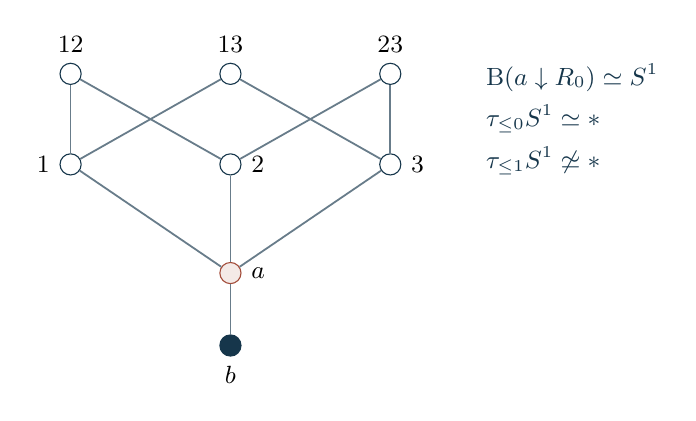
\begin{tikzpicture}[x=1.4cm,y=1.15cm,
 dot/.style={circle,draw=ink,fill=white,inner sep=2.7pt},
 edge/.style={draw=ink!65,line width=.65pt},
 every node/.style={font=\small}]
\node[dot,label=above:{$12$}] (e12) at (-1.45,3) {};
\node[dot,label=above:{$13$}] (e13) at (0,3) {};
\node[dot,label=above:{$23$}] (e23) at (1.45,3) {};
\node[dot,label=left:{$1$}] (v1) at (-1.45,2) {};
\node[dot,label=right:{$2$}] (v2) at (0,2) {};
\node[dot,label=right:{$3$}] (v3) at (1.45,2) {};
\foreach \v/\e in {v1/e12,v1/e13,v2/e12,v2/e23,v3/e13,v3/e23}
\draw[edge] (\v)--(\e);
\node[dot,draw=accent,fill=accent!12,label=right:{$a$}] (a) at (0,.8) {};
\node[dot,fill=ink,label=below:{$b$}] (b) at (0,0) {};
\foreach \v in {v1,v2,v3}\draw[edge] (a)--(\v);
\draw[edge] (b)--(a);
\node[align=left,text=ink] at (3.1,2.5)
 {$\B(a\downarrow R_0)\simeq S^1$\\[4pt]
  $\tau_{\leq0}S^1\simeq *$\\[4pt]
  $\tau_{\leq1}S^1\not\simeq *$};
\end{tikzpicture}
\caption{The eight-object poset $\Ccat_3$. The set-valued least resolver
contains every object except $a$; the space-valued least resolver also
requires $a$. This is a Hasse diagram: arrows point upward and transitive
arrows are omitted. The six incidence edges form a circle in the order
complex, despite crossings in the drawing.}
\label{fig:eight}
\end{figure}

For a set $A$, compatible assignments of its elements over a connected
indexing category are constant. Thus
\[
\limop_{\Pcat_3}\Delta A\cong A.
\]
There is no other omitted-object test, since only $a$ is omitted. Leastness
also has a direct description. Every maximal edge object must be present:
otherwise its comma category is empty. Each vertex must then be present:
if it is absent, the two incident maximal edges give a disconnected comma
category. All six objects are forced.

For a space $A$, however,
\[
\limop_{\Pcat_3}\Delta A\simeq\Map(S^1,A).
\]
The comparison selects constant loops. Taking $A=\K(\Z,1)$ produces
components indexed by $\Z$. The earlier resolution did not require this
loop data to vanish; it did not test it. Once groupoids become admissible,
the loop becomes visible. Adding $a$ gives the relevant comma category an
initial object and repairs the failure.

\begin{table}[htbp]
\centering
\begin{tabular}{@{}crrrr@{}}
\toprule
Indexing size & Sets & Groupoids & 2-types & 3-types\\
\midrule
$|\Ccat_3|=8$  &7&8&8&8\\
$|\Ccat_4|=16$ &11&15&16&16\\
$|\Ccat_5|=32$ &16&26&31&32\\
\bottomrule
\end{tabular}
\caption{Cardinalities of the least resolving full subposets. The starting
level and ambient indexing data are fixed within each row. Every row
eventually stabilizes at the whole indexing category.}
\label{tab:profiles}
\end{table}

These numbers are not a measurement of philosophical progress. They count
objects in a constructed poset. Their role is to distinguish senses of
resolution that ordinary notation could otherwise conceal.

\subsection{A nonconstant nine-object example}\label{sec:nonconstant}

The constant generation of the main family makes its comparison unusually
transparent. The same first jump survives genuinely nonconstant generation.
Start with $p<a<\Pcat_3$, and add an object $q$ with $q<1$, hence
$q<12,13$, and no other new comparisons. Here $1,2,3$ denote singleton
faces, while $12,13,23$ denote two-element faces. Let $D=\{p,q\}$;
its two objects are incomparable. For a pair $(A,B)$ of coefficient
objects, left extension produces the diagram $X=\Lan_D(A,B)$ with
\begin{equation}\label{eq:nonconstant}
\begin{array}{c|c}
\text{positions}&\text{value of }X\\\hline
p,a,2,3,23&A\\
q&B\\
1,12,13&A\sqcup B.
\end{array}
\end{equation}
The nonidentity transition maps are identities or the appropriate
coproduct inclusions. The lower comma categories for generation are
discrete, so these coproducts agree on old inputs in every coefficient
category. The diagrams are not constant, even when $A$ and $B$ are
connected nonempty types.

\begin{proposition}\label{prop:nonconstant}
In this nine-object poset the least full resolver of $D$ is $C\setminus
\{a\}$ for sets, and $C$ for all $k\geq1$, including unrestricted
spaces.
\end{proposition}

\begin{proof}
Taking $B=\varnothing$ and $A$ a two-element set forces all six faces:
the matching map at an edge is $A\to *$, and at a vertex it is the
diagonal $A\to A\times A$. Both fail to be bijective. Thus any
resolver already contains $D\cup\Pcat_3$.

To test the only remaining position $a$, restrict $X$ to
$J=\Pcat_3$. Color its $A$ summands by $0$ and its $B$ summands by
$1$, giving a natural map $X|_J\to\Delta_J\{0,1\}$. Since
$\B J\simeq S^1$ is connected, the limit of the latter is
$\{0,1\}$. The fiber of $\lim_JX$ over $0$ is the limit of the
constant $A$ diagram, hence $\Map(S^1,A)$. Its fiber over $1$ is
empty: that fiber diagram has empty values at $2,3,23$. Limits
preserve these pullbacks. Consequently
\[
M_aX=\limop_JX\simeq\Map(S^1,A),
\]
and its matching map is the constant-map comparison from $A$.
For sets it is always an equivalence. For $k\geq1$, take
$A=\K(\Z,1)$ and $B=*$: the comparison misses all nonzero winding
components. Apply \cref{prop:support,cor:arbitraryD}.
\end{proof}

This example isolates the two operations even without constant output
from left generation: every earlier generated diagram is preserved,
while the right reconstruction detects additional coherence.

\section{What changes, and what remains true}
\label{sec:change}

\subsection{Enlarging a test is not refuting its restricted version}

There is an easy but misleading way to describe the example: homotopy theory
reveals that the set-valued resolution was false. It does not. The
set-valued assertion remains true for every set. What changes is the range
of objects over which sufficiency is quantified.

\begin{proposition}[Persistence of the earlier tests]\label{prop:persistence}
In the setting of \cref{lem:criterion}, let $0\leq k\leq\ell\leq\infty$.
For every $A\in\mathcal V_k$, the resolution comparison is the same when
computed in $\mathcal V_k$ or in $\mathcal V_\ell$. Hence an
$\ell$-resolver is a $k$-resolver, while a $k$-resolver can fail to be an
$\ell$-resolver only on additional test objects.
\end{proposition}

\begin{proof}
The inclusion $\mathcal V_k\hookrightarrow\mathcal V_\ell$ is fully
faithful and preserves limits. Left extension from $D$ is constant in both
settings. Thus the pointwise right Kan extension and its unit agree on
$A\in\mathcal V_k$. An equivalence for all objects of the larger
category is, in particular, one for all objects of the smaller category.
\end{proof}

This proposition locates the result exactly. It does not exhibit a
contradiction between two answers to the same fully specified mathematical
question. It exhibits different answers to related questions whose
coefficient parameter was easily left implicit. The philosophical problem is
to determine when that parameter may legitimately remain fixed and when
the interpretation itself requires it to vary.

In particular, our main family is stronger as a test than the familiar
observation that a homotopy colimit can differ from an ordinary colimit.
That observation is relevant background \cite{Dugger}, and an elementary
example is recorded in the appendix. Here the source construction is
unchanged even on nondiscrete coefficients: $\Lan_D A$ is constant.
The defect lies in its reconstruction through a higher right Kan
extension. We have isolated the test of resolution from a possible change
in the generation of the object being tested.

More generally, let $i:\mathcal V\hookrightarrow\mathcal W$ be
fully faithful and preserve the relevant limits. If the canonical
comparison
\[
i\Lan_D^{\mathcal V} A\longrightarrow\Lan_D^{\mathcal W}(iA)
\]
is an equivalence for every old input $A$, then the generated resolution
units agree on those inputs. For finite $C$, this implies
$\Aup_{\mathcal V}(D)\subseteq\Aup_{\mathcal W}(D)$: a resolver in
$\mathcal W$ passes every old comparison, and hence contains the least
one in $\mathcal V$. The initial-singleton case satisfies this hypothesis,
as does the nine-object example because its generation uses coproducts.
The hypothesis is sufficient, and the next result shows why it cannot
simply be omitted.

\subsection{Changing generation can shrink a least resolver}
\label{sec:reversal}

Preservation of left generation is a substantive hypothesis in the
comparison of coefficients. Without it, the least resolving subset can
become smaller when the coefficient category becomes larger.

\begin{proposition}[Reversal when generation changes]
\label{prop:reversal}
Let $J$ be a nonempty finite poset, and put
\[
C=\{x\}\star J\star\{t\},\qquad D=J,\qquad U=J\star\{t\}.
\]
For finite $k\geq0$ let $T_k=\tau_{\leq k}\B J$, and put
$T_\infty=\B J$. Then
\[
\Aup_k(D)=
\begin{cases}
C,&T_k\simeq *,\\
U,&T_k\not\simeq *.
\end{cases}
\]
In particular, if $J=Q_{d+1}$ is the ordinal sum of $d+1$
two-element antichains, where $d\geq1$, then $|C|=2d+4$ and
\[
\Aup_k(D)=
\begin{cases}
C,&0\leq k<d,\\
C\setminus\{x\},&d\leq k\leq\infty.
\end{cases}
\]
\end{proposition}

\begin{proof}
For every $A:J\to\mathcal V_k$, its left extension $X=\Lan_D A$
has $X(x)=\varnothing$, restricts to $A$ on $J$, and has
$X(t)=\colim_J A$ with the canonical cocone. The terminal position
$t$ is mandatory at every coefficient level: taking the empty input
diagram gives the matching map $\varnothing\to *$ at $t$. The
positions in $D$ are mandatory by definition. It therefore remains
only to decide whether $x$ is mandatory.

Take the constant terminal input, and write
$F=(\Lan_D1)|_U$. Its restriction to $J$ is terminal and
$F(t)=T_k$. The canonical cocone represents the truncation map
$\eta:\B J\to T_k$, or the identity for $k=\infty$. A cone over
$F$ is a cone over its restriction to $J$, a point of $T_k$, and
compatibility with that cocone. Consequently
\[
\limop_U F\simeq
T_k\times_{\Map(\B J,T_k)}\{\eta\},
\]
where $T_k\to\Map(\B J,T_k)$ sends a point to the corresponding
constant map. By the universal property of truncation,
$\Map(\B J,T_k)\simeq\Map(T_k,T_k)$; under this equivalence,
$\eta$ is the identity and constant maps remain constant.
The displayed homotopy pullback is therefore nonempty exactly when
the identity of $T_k$ is homotopic to a constant, equivalently when
$T_k$ is contractible.

If $T_k$ is noncontractible, this limit is empty. For arbitrary
$A$, the unique map $A\to1$ induces
\[
\limop_U(\Lan_D A)|_U\longrightarrow\limop_U F=\varnothing.
\]
An object of spaces or truncated spaces admitting a map to the
empty object is itself empty. Thus the matching map at $x$ is
$\varnothing\to\varnothing$ for every input, and $U$ resolves $D$.
Together with the mandatory positions already identified, this
proves leastness.

If $T_k$ is contractible, $F$ is pointwise terminal on $U$, so its
limit is terminal. The matching map at $x$ for the terminal input
is then $\varnothing\to *$. Thus $x$ is also mandatory, and the
least resolver is $C$.

Finally, $\B Q_{d+1}\simeq S^d$. Its $k$-truncation is
contractible exactly for $0\leq k<d$, and is noncontractible for
finite $k\geq d$ and for unrestricted spaces. This proves the
last formula.
\end{proof}

For $d=1$, the least resolver has six objects for sets and five for
groupoids and all higher coefficients. This reverses the direction of
the main family's change. The reason is explicit: the terminal input
is generated with value $*$ at $t$ in sets and $S^1$ at $t$ in
groupoids. The main family and the nonconstant nine-object example
preserve their left generation on old inputs; this example does not.
The two behaviors concern different hypotheses.

\begin{table}[htbp]
\centering
\begin{tabular}{@{}lcrrl@{}}
\toprule
Six-object family & $|D|$ & Sets & Groupoids & Generation on old inputs\\
\midrule
$C'_2$ of \cref{prop:compact} & 1 & 5 & 6 & Preserved\\
Cone family of \cref{prop:reversal} & 4 & 6 & 5 & Changed\\
\bottomrule
\end{tabular}
\caption{Sizes of least resolvers in two different six-object posets.
Preserving generation guarantees monotonicity under the stated comparison
hypotheses; changing generation can reverse the inclusion.}
\label{tab:directions}
\end{table}

\subsection{A resolution profile}

For a fixed ambient indexing category, starting level, and admissible family,
call the sequence $k\mapsto\Aup_k(D)$ its \emph{resolution profile},
where the least levels exist. The expression is a name for the comparison
being studied, not a replacement for established cofinality terminology.

The profile contains more information than a single result. For the growing
families it shows both the validity of a restricted resolution and the first
expressive level at which it ceases to suffice. The reversal profile instead
loses a formerly essential position when generation changes.
In \cref{thm:main}, the failure has a
specified location, namely $a$, a specified shape, a wedge of spheres,
and a specified detecting coefficient, an Eilenberg--Mac Lane space. What
would otherwise be an unspecified demand for ``more structure'' becomes a
calculable request.

This also clarifies a distinction between erasure and invisibility. The
nerve is a circle already in the first example. Set-valued coefficients do
not turn that nerve into a contractible space; they are unable to distinguish
it from a point by the maps under consideration. The distinction untested by the comparison is
therefore relative to that test. To say that a result preserves everything
relevant is to say something about what counts as a relevant test, not only
about the construction of the result.

\subsection{Why leastness is not enough}

A least object is uniquely determined up to the relevant equivalence once
the ordered collection of candidates and its predicate of adequacy are
fixed. Leastness can therefore express a strong form of internal necessity.
In our family no alternative full subposet is smaller and still meets the
specified test. The matching-support calculation excludes all such alternatives.

Consider an explicit inference, introduced here as a claim to be tested,
not attributed to any of the authors discussed: if an enrichment keeps the
generation of the diagrams and every earlier resolution comparison intact,
then it also keeps their least adequate resolving level intact. The premise
is stronger than agreement on selected examples. It preserves the entire
old domain of comparisons. Yet \cref{prop:persistence,thm:main} jointly
refute the conclusion, with arbitrarily long finite chains of different
least levels.

What survives is correctness on the earlier domain; what fails is its
sufficiency to determine the least adequate reconstruction on the enlarged
domain. This distinction is not a discrepancy between an informal reading
and a formal calculation. It occurs between formally stated properties,
with fixed indexing data and fixed generation. Leastness combines an order
of candidates with a predicate of adequacy. Persistence of old comparisons
preserves one part of the predicate's evidence without establishing the
completeness of its range.

For a reconstruction of dialectical necessity, the consequence is conditional
but exact. If its explanatory commitments give a reason to admit additional
tests, continued agreement on all earlier tests does not by itself secure
its earlier leastness claim. It must justify the original test domain,
prove a transport result, or accept a changed least resolution. If no such
reason is given, our theorem supplies a possible comparison rather than a
refutation. This is the distinction between a useful external analysis and
an internally demanded revision to which we now turn.

\section{Determinate preservation as an interpretive requirement}
\label{sec:preservation}

\subsection{A criterion with a limited demand}

We propose the following requirement for a mathematical reconstruction of
sublation:
\begin{quote}
State the relations claimed to represent the mediation and the distinctions
whose retention constitutes the proposed preservation; show how the
resolving construction retains them; and justify the treatment
of distinctions that become detectable under the reconstruction's own
licensed changes of language.
\end{quote}
This requirement of \emph{determinate preservation} is our methodological
proposal. It is not a quotation from Hegel or a theorem of category theory.
Its motivation is that preservation needs a determinate content if it is to
play an explanatory role. The theorem supplies an exact case in which an
unqualified preservation claim would conceal a choice.

The demand is intentionally weaker than invariance under every enrichment.
Not every new formal distinction deserves philosophical recognition. A set-based
model can be exactly appropriate for a question about ordinary
classification. A groupoid model may be appropriate when identifications
and automorphisms matter. The requirement is to defend this choice in
relation to the interpreted material, not to rank models by how much
machinery they contain.

A change of test becomes relevant in at least three distinguishable ways.
The reconstruction may itself use the additional structure to explain the
passage; its claimed applications may require that structure; or a close
reading may show that its original tests identify distinctions it needs to
retain. These are warrants that can be contested with textual and
mathematical evidence. Merely knowing that groupoids are available is not
such a warrant. Conversely, declaring that only sets are admissible does
not settle the issue if the explanatory argument already invokes coherent
identity. The present theorem diagnoses consequences once a warrant is
given; it does not manufacture that warrant.

Nor does the requirement insist that every revision add more objects.
In the generation-preserving families the least resolver grows;
\cref{prop:reversal} shows that a change of generation can instead
make it shrink. Another model might revise its equivalences, its morphisms,
or its admissible tests instead. The general lesson is about explicit
dependence on representational choices; the particular repairs in a
constructed poset do not constitute a universal recipe for dialectic.

\subsection{Retention without identity of status}

The philosophical attraction of sublation is that something can persist
without retaining its former independence. A categorical reconstruction can
give this thought more than one precise form. An object may occur as the
image of an embedding, as a retract, as a component of gluing data, or as
the value of a modality. These are different modes of dependence. Their
differences should be used rather than obscured by a common label.

Our resolution condition does one specific job: an earlier skeletal object
is recoverable through a later right extension. This captures a relation of
recoverability and changed presentation. It does not independently capture
every philosophical sense of negation, nor does it show that the earlier
concept has criticized itself. The model is informative because its
achievement can be stated exactly.

There is also a limit to the familiar picture of preservation as storage.
Keeping a copy of every earlier object need not preserve the relations
that made those objects what they were. In homotopy theory, retaining points
while suppressing paths can alter the character of the object. In an
inferential account, retaining sentences while changing which consequences
they license can alter their content. The analogy between these cases is
methodological, not an identification of paths with inferences. Both require
the interpretation to specify the relations its preservation concerns.

\subsection{What is established in the content, and what is available to us}

The distinction in Hegel's discussion of determinate being is especially
instructive. In online paragraph 193, a determination may be available to
our reflection before it is established as part of the concept's own
development. Such a comparison can elucidate or anticipate; that does not
give it the status of a ground of the transition \cite{HegelDasein}.

The author's running commentary, distinct from the earlier interactive
map, foregrounds this problem in its first two readings
\cite{AutioCommentary}. Its distinction between what is available
``for us'' and what has been posited within the development helps formulate
the interpretive demand. It is a statement of the problem, not independent
evidence that a particular reconstruction meets it.

Applied to this paper, the distinction asks why a coefficient enrichment
belongs to the represented content rather than only to our means of
investigating it. The answer cannot be that the richer formalism exists.
Nor can it be that the enrichment has produced an interesting theorem.
Those facts justify studying the comparison, but they do not determine
its interpretive status. A close reading must identify the relevant demand
of the content; a mathematical preservation theorem must then establish
what the chosen formal correlate achieves.

This yields an interpretation audit with a definite result. Measured
against the demands drawn from the becoming passage, our formal calculation
establishes recoverability and least repair only for its stipulated
mathematical data. It does not supply the moments'
self-transformation or explain their altered significance. For the status
of the coefficient category, it supplies a sensitivity result but no
immanent warrant for enrichment. The mathematical result is therefore
philosophically useful in an elucidatory role, while its promotion to a
derivation would require evidence it does not provide.

\subsection{Immanence and the status of the formal language}

Hegel's final discussion of method presents the relation between method and
content as internal rather than as the application of an independently
chosen technique \cite{HegelIdea}. A mathematical reconstruction necessarily
begins with some formal resources. It cannot escape that fact by describing
those resources as universal. It can, however, make their role an object
of the reconstruction rather than leaving it as an unexplained background.

Hentrup's account of rational proof supplies an independent philosophical
comparator. In section II, geometric demonstration can establish a
necessity belonging to its object while its progression remains the
prover's activity. In sections V--VI, rational proof requires mutual
mediation in which the terms' identities develop, rather than reciprocal
support between fixed terms \cite{Hentrup}. On this reading, the
difference between valid demonstration and adequate mediation is already
a substantive Hegelian problem. Our contribution is not to discover that
difference, but to make two dependencies of a formal reconstruction
calculable: the tests that determine its least resolver and the
relations whose interpretation remains to be justified.

The resolution profile offers one finite way to do so. The coefficient
category is first a parameter of the model; the profile then shows how
the model's verdict depends on it. This does not reproduce Hegel's claim
that the method determines itself. It provides a disciplined partial
analogue: the consequences of the choice of method are brought into the
argument and can be evaluated. A stronger claim of self-determination
would require additional work explaining why the sequence of admissible
tests is generated by the subject matter rather than chosen by us.

The gap should remain visible. Our theorem can force the next resolving
level \emph{if} the next coefficient category is admitted. It does not force
the admission of that category. Confusing these two steps would repeat,
at a higher level, the very substitution of external comparison for internal
development that the reconstruction is meant to illuminate.

\subsection{A reader audit: stable profiles and different relations}
\label{sec:readeraudit}

Coefficient variation is not the only choice a reconstruction makes.
The author's earlier interactive reader \cite{AutioReader} supplies a
concrete case in which to distinguish it from the choice of indexing
relations. The reader locates sections within larger sections and
opens their associated passages. Containment and succession are both
legitimate editorial relations. Neither, by itself, establishes the
dependence by which one determination generates another.

Consider two explicitly stipulated encodings of the same positions.
In one, an ancestor is below its descendants in a rooted tree. In the
other, the positions are totally ordered by a traversal compatible
with that ancestry. A synthetic book-header root is first in both.
It is an editorial device, not an identification with Pure Being;
likewise the second order records succession, not implication.

\begin{proposition}[A limit of the profile diagnostic]\label{prop:treechain}
Let $T$ be a finite rooted tree with root $b$, with at least two
children at every nonleaf vertex. Let $L$ be a total order on the same
vertex set extending the ancestor order, and write $t$ for its last
vertex. For $D=\{b\}$ and every $0\leq k\leq\infty$,
\begin{equation}\label{eq:treechain}
\Aup_k^T(D)=T,\qquad \Aup_k^L(D)=\{b,t\}.
\end{equation}
Thus both profiles are invariant under coefficient enrichment, although
their least subsets can differ by arbitrarily many objects.
\end{proposition}

\begin{proof}
At a leaf of $T$ the strict upper interval is empty. At a nonleaf it is
the disjoint union of the descendant subtrees rooted at its children.
Each component has an initial object, so its nerve is contractible;
there are at least two such components. Every vertex therefore belongs
to $E_k(T)$ at every $k$. In $L$, only $t$ has empty strict upper
interval; at every earlier vertex that interval has a least element.
Hence $E_k(L)=\{t\}$. Apply \cref{thm:intrinsic} and add the required
starting object $b$. Finite branching trees can have arbitrarily many
vertices.
\end{proof}

\begin{figure}[htbp]
\centering
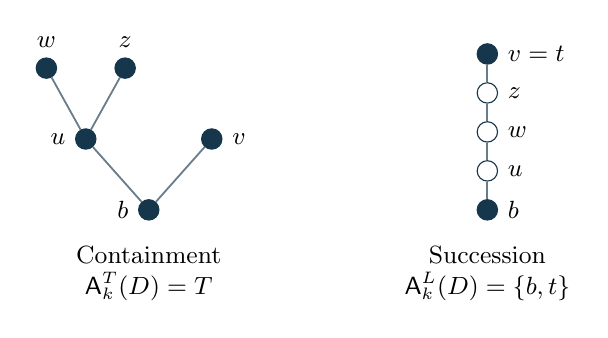
\begin{tikzpicture}[x=1cm,y=.9cm,
 kept/.style={circle,draw=ink,fill=ink,inner sep=2.6pt},
 omitted/.style={circle,draw=ink,fill=white,inner sep=2.6pt},
 edge/.style={draw=ink!65,line width=.65pt},
 every node/.style={font=\small}]
\node[kept,label=left:{$b$}] (tb) at (0,0) {};
\node[kept,label=left:{$u$}] (tu) at (-.8,1) {};
\node[kept,label=right:{$v$}] (tv) at (.8,1) {};
\node[kept,label=above:{$w$}] (tw) at (-1.3,2) {};
\node[kept,label=above:{$z$}] (tz) at (-.3,2) {};
\foreach \s/\t in {tb/tu,tb/tv,tu/tw,tu/tz}
\draw[edge] (\s)--(\t);
\node[align=center] at (0,-.9) {Containment\\$\Aup_k^T(D)=T$};
\node[kept,label=right:{$b$}] (lb) at (4.3,0) {};
\node[omitted,label=right:{$u$}] (lu) at (4.3,.55) {};
\node[omitted,label=right:{$w$}] (lw) at (4.3,1.1) {};
\node[omitted,label=right:{$z$}] (lz) at (4.3,1.65) {};
\node[kept,label=right:{$v=t$}] (lv) at (4.3,2.2) {};
\foreach \s/\t in {lb/lu,lu/lw,lw/lz,lz/lv}
\draw[edge] (\s)--(\t);
\node[align=center] at (4.3,-.9) {Succession\\$\Aup_k^L(D)=\{b,t\}$};
\end{tikzpicture}
\caption{Two stipulated orders on the same positions. Filled vertices
are in the least resolver for every coefficient level. The invariance
of both profiles does not decide which relation, if either, models
the intended mediation. Arrows in these Hasse diagrams point upward.}
\label{fig:treechain}
\end{figure}

The active reader contains 120 positions in four displayed depths.
After excluding its one unnamed placeholder and adding the synthetic
root, there are 120 named-or-root positions. Every internal vertex
still has at least two children. The proposition therefore applies
to these proposed encodings. These counts describe the inspected
editorial data; they assert neither a canonical inventory of Hegelian
categories nor a mathematical structure derived from the text.

The contrast supplies a limit on our own diagnostic. Invariance of a
resolution profile is insufficient for interpretive adequacy. The
opposed leastness verdicts here are explained by branching and
terminality before any philosophical content is assigned to the
labels. This does not make either encoding defective: it specifies
what each achieves. In this case the unsettled choice concerns
relations; in the Boolean family the relations are fixed and the
varying choice concerns tests. The two choices require distinct
arguments.

A passage-grounded extension would therefore distinguish containment,
succession, and argued dependence, recording textual evidence for the
latter instead of silently replacing it with either of the former.
Composites and identifications between dependency paths would require
further justification before a category or higher category is claimed.
The present paper does not invent those relations in order to find
Hegelian loops. It identifies what such an extension would need to
establish before a homotopy calculation acquired that interpretation.

\subsection{A mathematical reading need not be a reduction}

The distinction between orientation and derivation has a direct textual
basis. In the final discussion of method, Hegel permits an advance survey
of the whole while denying that division into its already specified parts
establishes their transition (online paragraph 1813). The author's earlier
interactive reader \cite{AutioReader} makes this distinction concrete:
its hierarchy locates moments and opens the corresponding passages.
Such navigational success need not claim to establish their mediation.
Nor does a circular display by itself realize the return through mediation
described in paragraph 1814. A formal interpretation must say which of
these achievements it intends.

There is also a challenge to our own procedure. Paragraph 1812 rejects
the claim that criticism of cognition's instrument enjoys an automatic
priority over engagement with the subject matter: that criticism has
presuppositions of its own \cite{HegelIdea}. Determinate preservation
should therefore operate within the examination of a reconstruction,
rather than as a preliminary tribunal that settles its possibility in
advance. The test must answer to the content it claims to illuminate.
Our theorem identifies a dependence to be justified; it neither supplies
a presuppositionless standpoint nor decides that justification before
the interpretation has been attempted.

The value of a mathematical reading is not exhausted by translation into a
fixed formal calculus. It can reveal a question that was difficult to state,
separate claims previously run together, and supply counterexamples to an
overextended argument. Here the precise separation is between the
existence of a least resolver and the justification of its criterion of
resolution.

This supports a reciprocal rather than a reductive relation between
philosophy and mathematics. The philosophical concern with retention
motivates a comparison of coefficients; the mathematical comparison then
forces the philosophical concern to become more specific. Neither side
receives authority simply by borrowing the other's vocabulary. What matters
is whether the encounter changes the questions that can responsibly be
asked and the answers that can be defended.

\section{Contemporary alternatives and adjacent results}
\label{sec:literature}

\subsection{Progression, contradiction, and logical form}

Priest's model uses paraconsistent logic, but also specifies a concrete
retention condition: introducing the new predicate leaves the old
vocabulary's extensions and anti-extensions unchanged
\cite[section 3]{Priest}. In section 6 he expressly limits the aim to the
logical structure of progression, rather than an explanation of why a
progression occurs. These are precedents for specifying preservation and
scope, not errors our theorem corrects. His retention condition is
stipulated in the construction; ours is Kan-extension recoverability
with a proved leastness profile. Neither identification alone establishes
its adequacy to the text.

An adjunction does not assert $P\wedge\neg P$, and a homotopical
obstruction does not license or reject explosion. A useful comparison
must therefore identify shared explanatory tasks before treating
paraconsistency and modal adjunctions as competing answers to one
question.

Yang's published abstract distinguishes the accuracy of describing
dialectical progression from the ability to explain it \cite{Yang}.
This distinction is congenial to our separation of retention,
determination, and necessity. We do not rely on a detailed reconstruction
of Yang's argument, whose full text was not available for this study.
Our mathematical result provides an independent instance of the general
difference: a diagram can describe a proposed transition without
settling why its adequacy criterion is the appropriate one.

Kolman's account treats Hegel's relation to logical form through the
reconsideration of fixed determinations rather than the mere addition of
one more logical form \cite{Kolman}. Our proposal shares that concern
with the status of a formal standpoint, while giving it a different
technical expression. Changing coefficients does not model a history of
logic. It gives a controlled comparison in which what a formalism can
detect becomes part of the account of its verdict.

Brown offers a positive example of making preservation explicit.
Definition 2.6 calls a morphism $f:X\to Y$ of incompatibility frames
conservative when every finite multiset $\Gamma$ is incompatible in $X$
exactly when $f(\Gamma)$ is incompatible in $Y$. Proposition 2.1 proves
this property for the adjunction unit; the signed construction inherits
it in section 3.2 \cite{Brown}. The universal construction thus has a
separately stated preservation achievement. It differs from our
Kan-extension recoverability. The methodological point is that specifying
an adjunction and specifying what it retains are distinguishable tasks.

\subsection{What recent Aufhebung calculations already achieve}

The work of Kennett, Riehl, Roy, and Zaks computes actual skeletal and
coskeletal bounds in ordinary presheaf topoi \cite{KennettEtAl}. Their
results show why an unspecified ``next dimension'' is not an adequate
description of Aufhebung. The precise bound depends on the indexing
category, and low-dimensional cases require attention.

The recent solution by Hora, Kamio, and Maehara to Lawvere's fourth
problem computes the relation for symmetric simplicial sets
\cite{HoraEtAl}. This removes that calculation from the list of open
targets. Our family changes a different parameter: its indexing category
is fixed while its coefficients vary. The elementary topology involved
does not make it a replacement for the substantially deeper combinatorics
of their theorem.

Menni's work on the least subtopos containing the discrete skeleton of
$\Omega$ shows the power of replacing a large containment condition by
a distinguished generator \cite{Menni}. It also makes essentiality a
substantive issue. One cannot freely identify a least subtopos with a
least essential resolving level. This is why our higher theorem names
its admissible full-subcategory levels explicitly instead of relying on
an unstated lattice classification.

Dey--Lesnick and Br\"ustle--Desrochers--Leblanc address the least
full subposets needed for ordinary limit or colimit computation
\cite{DeyLesnick,BrustleEtAl}. They are direct antecedents of the
$k=0$ upper-interval mechanism, while their treatment of nonfull
relation-sparse subposets optimizes a different admissible class. Our
calculation combines a truncated version of this mechanism with explicit
sphere obstructions to compare coefficients. It does not reopen the
ordinary least-full-subposet problem as if that literature did not exist.

\subsection{What a checked construction preserves}

DeBruce's Cubical Agda tutorial offers a useful contemporary example
because it places explicit limitations beside its formal declarations.
Chapter 4 introduces a higher inductive type \texttt{Becoming} with two
points, \texttt{being} and \texttt{nothing}, and a path between them
\cite{DeBruce}. These points are new inhabitants of a common carrier.
They are not the unit and empty types used for Being and Nothing in
Chapter 2. The distinction matters: a path between those earlier types
would transport an inhabitant of the unit type into the empty type.
The consistent construction therefore depends on changing what is
related, not simply on replacing judgmental equality with path equality.
An interpretation must explain which roles of the earlier assignments
survive this change.

The same chapter declares an \texttt{Aufhebung} record containing a
higher unity and a function from the lower moment to the higher. It
explicitly leaves an instance unconstructed and acknowledges missing
compatibility requirements; it supplies no leastness theorem. These are
useful limits on the achievement, not reasons to dismiss it. The tutorial
makes an interpretive audit concrete: naming, providing a structure,
retaining a specified property, and proving minimality are distinguishable
accomplishments. We assess the inspected declarations and their
interpretation; we have not independently rerun that project's Agda build.

\subsection{Higher modal semantics is infrastructure, not a transfer theorem}

Uemura's internal languages for diagrams of infinity-logoses connect
modalities, gluing, and higher categorical semantics \cite{Uemura}.
Shulman's multimodal adjoint type theory provides a systematic treatment
of modal adjunctions and their semantics \cite{Shulman}. Myers and Riley
study multiple commuting cohesions \cite{MyersRiley}. These works make
the higher setting substantially more precise than an informal instruction
to replace sets by types.

The computational side is also important. Gratzer's normalization result
relates type checking to equality in the chosen mode theory
\cite{Gratzer}; the combination of cubical and multimodal type theory
provides another route toward expressing homotopical modal arguments
\cite{AagaardEtAl}. None of these metatheorems selects the mode theory
appropriate to Hegel, and none by itself says that a given set-valued
resolution has the same least solution in spaces. They supply languages
in which such questions can be asked rigorously.

Protin's recent discussion of Hegel and topology offers mathematical
illustrations and hermeneutic proposals \cite{Protin}. The contrast with
our purpose is one of task: we isolate a preservation claim and calculate
its failure of transport. An illustration can illuminate a passage without
claiming to establish a universal property; a universal property can be
proved without establishing that the passage has been interpreted correctly.
The distinction protects both kinds of work from exaggerated expectations.

\section{Conclusion: the conditions of a necessary transition}
\label{sec:conclusion}

The finite families give definite mathematical answers. A fixed initial
level can have successively different least resolutions when its admissible
coefficients range from sets through higher truncated spaces. The entire
sequence is calculable; its obstructions are explicit; its leastness holds
against every full-subcategory competitor. The earlier answer remains
true within its domain, while a richer domain detects what it did not test.
When generation changes as well, the reversal family shows that the least
resolver can instead shrink. Preserving the earlier generation is therefore
a substantive condition on a comparison, not a harmless convention.

The reader audit supplies the converse restraint. Containment and
succession, encoded on the same positions, can yield sharply different
least resolvers while both profiles remain coefficient-invariant.
Robustness under a change of tests is therefore no certificate that the
relations being tested express the intended mediation. Together the
examples separate two tasks: accounting for the admitted relations,
and accounting for the domain over which their adequacy is tested.

For a mathematical reading of Hegel, the result recommends neither a
retreat from formalization nor an unqualified preference for higher
structures. It recommends a more demanding account of preservation.
The interpretation must identify the content of what survives, the
equivalences under which it survives, and the tests by which its survival
is judged. As the interpretation proceeds, those choices must answer
to the text and explanatory task. A universal property can then help
explain the conditional necessity of its result without being asked
to justify the representation by itself.

Lawvere's approach is especially valuable because it permits this demand
to become mathematics. A proposed resolution can fail, and the failure
can have a shape. In our example that shape is a sphere invisible to one
coefficient category and visible to the next. The philosophical lesson
is not that every hidden sphere is a dialectical moment. It is that a
formal account of a necessary transition owes an account of what its
notion of necessity can see.

\begingroup
\small\raggedright
\begin{thebibliography}{99}
\addcontentsline{toc}{section}{References}

\bibitem{HegelSublation}
G.~W.~F. Hegel, \emph{Science of Logic}, Doctrine of Being, section 1,
chapter 1, C.3, remark on the expression ``To Sublate'' (online
paragraph numbering 184--187).
\url{https://www.marxists.org/reference/archive/hegel/works/hl/hlbeing.htm}.

\bibitem{KennettEtAl}
C. Kennett, E. Riehl, M. Roy, and M. Zaks, Levels in the toposes of
simplicial sets and cubical sets, \emph{Journal of Pure and Applied
Algebra} \textbf{215} (2011), 949--961.
\href{https://doi.org/10.1016/j.jpaa.2010.07.002}{doi:10.1016/j.jpaa.2010.07.002}.
Author-hosted text: \url{https://math.jhu.edu/~eriehl/levels.pdf}.

\bibitem{Menni}
M. Menni, The least subtopos containing the discrete skeleton of
$\Omega$, \emph{Theory and Applications of Categories} \textbf{42}
(2024), no.~8, 172--179.
\url{https://arxiv.org/abs/2408.00514}.

\bibitem{Du}
P. Du, Reshaping limit diagrams and cofinality in higher category
theory, arXiv:2308.01798, version 5 (2023), especially section 6.
\url{https://arxiv.org/html/2308.01798v5}.

\bibitem{DeyLesnick}
T.~K. Dey and M. Lesnick, Limit computation over posets via minimal
initial functors, arXiv:2601.00209, version 2 (20 January 2026).
\url{https://arxiv.org/html/2601.00209v2}.

\bibitem{HegelIntro}
G.~W.~F. Hegel, \emph{Science of Logic}, Introduction, ``General Notion
of Logic,'' especially the discussion of determinate negation and method
(online paragraph numbering 33--34 and 62--63). English text in the
Marxists Internet Archive:
\url{https://www.marxists.org/reference/archive/hegel/works/hl/hlintro.htm}.
For a modern edition see \emph{The Science of Logic}, trans. and ed.
George di Giovanni, Cambridge University Press, 2010.

\bibitem{Lawvere1996}
F.~W. Lawvere, Unity and identity of opposites in calculus and physics,
\emph{Applied Categorical Structures} \textbf{4} (1996), 167--174.
\href{https://lawverearchives.com/wp-content/uploads/2024/12/1996-unity-and-identity-of-opposites-in-calculus-and-physics.pdf}{Lawvere Archives full text}.

\bibitem{HegelBecoming}
G.~W.~F. Hegel, \emph{Science of Logic}, Doctrine of Being, section 1,
chapter 1, C.2--3, ``Moments of Becoming'' and ``The Sublation of
Becoming'' (online paragraph numbering 176--183).
\url{https://www.marxists.org/reference/archive/hegel/works/hl/hl083.htm}.

\bibitem{nLabLogic}
nLab contributors, Science of Logic, collaborative online article,
revision 283 (13 June 2025), consulted 22 October 2026.
\url{https://ncatlab.org/nlab/revision/Science+of+Logic/283}.

\bibitem{nLabAufhebung}
nLab contributors, Aufhebung, collaborative online article,
revision 117 (27 December 2025), consulted 22 October 2026.
\url{https://ncatlab.org/nlab/revision/Aufhebung/117}.

\bibitem{Praehauser}
A. Pr\"ahauser, \emph{Hegel in Mathematics}, repository manuscript,
consulted 22 October 2026, section on Aufhebungen.
\url{https://github.com/nameiwillforget/hegel-in-mathematics}.

\bibitem{HegelDasein}
G.~W.~F. Hegel, \emph{Science of Logic}, Doctrine of Being, section 1,
chapter 2, A(a), ``Determinate Being in General,'' particularly the
distinction between determinations of the concept and external reflection.
\url{https://www.marxists.org/reference/archive/hegel/works/hl/hl109.htm}.

\bibitem{RiehlVerity}
E. Riehl and D. Verity, The theory and practice of Reedy categories,
\emph{Theory and Applications of Categories} \textbf{29} (2014),
no.~9, 256--301, especially section 3.
\url{https://emilyriehl.github.io/files/reedy.pdf}.

\bibitem{BrustleEtAl}
T. Br\"ustle, J. Desrochers, and S. Leblanc, Generalized rank via
minimal subposet, arXiv:2510.10837, version 5 (17 August 2026),
to appear in \emph{Linear Algebra and its Applications}.
\url{https://arxiv.org/html/2510.10837v5}.

\bibitem{BarmakMinian}
J.~A. Barmak and E.~G. Minian, One-point reductions of finite spaces,
$h$-regular CW-complexes and collapsibility,
\emph{Algebraic \& Geometric Topology} \textbf{8} (2008), 1763--1780.
\href{https://doi.org/10.2140/agt.2008.8.1763}{doi:10.2140/agt.2008.8.1763}.

\bibitem{BarmakMinimal}
J.~A. Barmak and E.~G. Minian, Minimal finite models,
\emph{Journal of Homotopy and Related Structures} \textbf{2}
(2007), no.~1, 127--140.
\url{https://mate.dm.uba.ar/~jbarmak/minimalrevised.pdf}.

\bibitem{Marques}
J. Marqu\`es, A criterion for categories on which every Grothendieck
topology is rigid, \emph{Applied Categorical Structures} \textbf{33}
(2025), article 37.
\href{https://doi.org/10.1007/s10485-025-09833-z}{doi:10.1007/s10485-025-09833-z}.
The published version is used; the arXiv version flags a corrected claim
about Cauchy completeness.

\bibitem{Dugger}
D. Dugger, A primer on homotopy colimits, expository manuscript.
\url{https://ncatlab.org/nlab/files/Dugger-PrimerHomotopyColimits.pdf}.

\bibitem{HegelIdea}
G.~W.~F. Hegel, \emph{Science of Logic}, Doctrine of the Concept,
section 3, chapter 3, ``The Absolute Idea,'' especially the discussion
of method (online paragraph numbering 1784--1785 and 1812--1814).
\url{https://www.marxists.org/reference/archive/hegel/works/hl/hlabsolu.htm}.

\bibitem{Hentrup}
M. Hentrup, Hegel's theory of rational proof, \emph{Hegel Bulletin},
First View (published online 26 November 2025), 1--23.
\href{https://doi.org/10.1017/hgl.2025.10083}{doi:10.1017/hgl.2025.10083}.

\bibitem{AutioReader}
P.~M. Autio, \emph{A Map of Hegel's Science of Logic}, interactive
reader (2015; revising a 2012 version), consulted 22 October 2026.
The site credits A.~V. Miller's translation through A.~Blunden's
transcription. \url{https://autio.github.io/projects/scienceoflogic/}.

\bibitem{AutioCommentary}
P.~M. Autio, \emph{Hegel Reader: The Science of Logic---Running
Commentary} (2026), readings of 6 and 7 June; consulted 22 October 2026.
\url{https://autio.github.io/hegel-reader/}.

\bibitem{Priest}
G. Priest, The logical structure of dialectic, \emph{History and
Philosophy of Logic} \textbf{44} (2023), no.~2, 200--208.
\href{https://doi.org/10.1080/01445340.2023.2182584}{doi:10.1080/01445340.2023.2182584}.
Author-hosted text: \url{https://grahampriest.net/?ddownload=8696}.

\bibitem{Yang}
C. Yang, On the formalization of Hegel's dialectical logic,
\emph{History and Philosophy of Logic} \textbf{47} (2026), no.~3,
340--347; first published online 17 November 2025.
\href{https://doi.org/10.1080/01445340.2025.2585746}{doi:10.1080/01445340.2025.2585746}.
The comparison in this manuscript is limited to the publisher's abstract.

\bibitem{Kolman}
V. Kolman, Hegel and the logical form, \emph{Logic and Logical
Philosophy} \textbf{32} (2023), no.~3, 383--401.
\href{https://doi.org/10.12775/LLP.2023.010}{doi:10.12775/LLP.2023.010}.

\bibitem{Brown}
K. Brown, A category-theoretic reconstruction of logical expressivism,
arXiv:2605.24796 (2026).
\url{https://arxiv.org/html/2605.24796v1}.

\bibitem{HoraEtAl}
R. Hora, Y. Kamio, and Y. Maehara, Lawvere's fourth open problem:
Levels in the topos of symmetric simplicial sets, arXiv:2503.03439,
version 2 (25 March 2025).
\url{https://arxiv.org/html/2503.03439v2}.

\bibitem{DeBruce}
D. DeBruce, \emph{Hegel's Logic in Cubical Agda}, tutorial implementation
(2026), chapters 2 and 4, consulted 22 October 2026.
\href{https://github.com/ddebruce/hegel-agda/blob/40cf024b731494db806801dcf0948b2f65d52331/book/src/ch04-unity-aufhebung.lagda.md}{Chapter 4 source at inspected commit}.
\url{https://ddebruce.github.io/hegel-agda/}.

\bibitem{Uemura}
T. Uemura, Homotopy type theory as internal languages of diagrams of
$\infty$-logoses, in \emph{FSCD 2023}, LIPIcs \textbf{260}, article 5,
2023. \href{https://doi.org/10.4230/LIPIcs.FSCD.2023.5}{doi:10.4230/LIPIcs.FSCD.2023.5}.

\bibitem{Shulman}
M. Shulman, Semantics of multimodal adjoint type theory,
\emph{Electronic Notes in Theoretical Informatics and Computer
Science} \textbf{3} (2023), article 12300.
\href{https://doi.org/10.46298/entics.12300}{doi:10.46298/entics.12300}.
Preprint: arXiv:2303.02572, version 5 (18 November 2023).
\url{https://arxiv.org/html/2303.02572v5}.

\bibitem{MyersRiley}
D.~J. Myers and M. Riley, Commuting cohesions, arXiv:2301.13780
(2023). \url{https://arxiv.org/abs/2301.13780}.

\bibitem{Gratzer}
D. Gratzer, Normalization for multimodal type theory,
\emph{Logical Methods in Computer Science} \textbf{22} (2026),
no.~1, article 27.
\href{https://doi.org/10.46298/lmcs-22(1:27)2026}{doi:10.46298/lmcs-22(1:27)2026}.
Preprint: \url{https://arxiv.org/html/2301.11842v4}.

\bibitem{AagaardEtAl}
F.~L. Aagaard, M.~B. Kristensen, D. Gratzer, and L. Birkedal,
Unifying cubical and multimodal type theory, \emph{Logical Methods in
Computer Science} \textbf{20} (2024), no.~4, article 25, 1--34.
\url{https://cpv.au.dk/pdfs/2024-cubical-mtt-final.pdf}.

\bibitem{Protin}
C. Protin, Hegel and modern topology, arXiv:2501.02367,
version 9 (25 June 2026).
\url{https://arxiv.org/html/2501.02367v9}.

\end{thebibliography}
\endgroup

\appendix
\section{The preliminary left-extension obstruction}
\label{app:left}

An elementary calculation motivated the main construction but should be
distinguished from it. Let $J=\Pcat_3$, and add a terminal object $t$ to
obtain $C$. For the constant singleton diagram $1:J\to\Set$,
\[
(\Lan_J^{\Set}1)(t)=\colim_J 1=1.
\]
For the same discrete-valued diagram in spaces,
\[
(\Lan_J^{\Spc}1)(t)\simeq\hocolim_J *\simeq\B J\simeq S^1.
\]
Thus the natural comparison from the space-valued extension to the
discrete image of the set-valued extension is not an equivalence.
This is a standard example of the topology retained by a homotopy
colimit \cite{Dugger}. It is not, on its own, a failure of an
Aufhebung relation. The main family isolates the latter kind of issue
by making its left extension constant in every coefficient category.

More generally, for a set-valued diagram $F$ on an ordinary category $J$,
the homotopy colimit of its discrete image is the classifying space of
its category of elements. The ordinary colimit records the connected
components of that category. The comparison is an equivalence precisely
when each component has contractible classifying space. This familiar
description is useful for checking where a discrete-to-homotopy comparison
can fail; it must not be promoted into a general contractibility test
based on homology alone.

\section{Reproducibility and the status of verification}
\label{app:verification}

The accompanying program \texttt{verify\_family.py} uses only the Python
standard library. It constructs order complexes, represents boundary
matrices as bitsets, and computes their ranks over $\mathbb F_2$ by
Gaussian elimination. The report is saved as
\texttt{verification.json}. Run it with:
\begin{quote}
\texttt{python verify\_family.py}
\end{quote}

For $N=3$, the program examines all $2^7=128$ full subposets
containing $b$. For $N=4$, it examines all $2^{15}=32{,}768$. At each
omitted object it tests the necessary condition of connectedness and
vanishing reduced homology through degree $k$ in the comma nerve. The
resulting candidate counts are:
\begin{center}
\begin{tabular}{@{}crrr@{}}
\toprule
$N$ & $k=0$ & $k=1$ & $k=2$\\
\midrule
3 & 2 & 1 & 1\textsuperscript{\,a}\\
4 & 32 & 2 & 1\\
\bottomrule
\end{tabular}\par
\smallskip
{\footnotesize\textsuperscript{a}The script exhausts $k=0,1$ for $N=3$;
the last value follows from the identity-only result.}
\end{center}
In each enumerated case, the homological necessary conditions agree with
containment of the predicted least level. This agreement is supplementary
evidence. It does not generally turn a necessary homological test into a
sufficient homotopical one. The proof of sufficiency is the wedge
calculation in the text.

For $N=3,4,5,6$, the program additionally checks the predicted homology
of every proposed proper least resolver at $a$, verifies the expected
failure at the next homological degree, and tests deletion of each
mandatory face even when all other objects are available. It does not
enumerate every subposet for $N=5$ or $6$.

The additional program \texttt{verify\_matching.py} independently
enumerates finite limits as compatible tuples. It examines every
naturally labelled poset on up to four objects and every functor whose
object sets have cardinalities $0,1,2$, checking all full reconstruction
subsets. It performs 121,774 comparisons across 7,766 diagrams; the
four-object cases include 5,763 diagrams with varying cardinalities.
These are direct Set-valued checks of \cref{prop:support}, not nerve
or homology tests. The program \texttt{verify\_nonconstant.py} checks
all 128 admissible subsets of the nine-object example against nine
input pairs of finite sets, performing 1,152 reconstruction checks.

For the shrinking family, \texttt{verify\_reversal.py} enumerates
553 Set-valued diagrams on $Q_2$, forms their quotient-set colimits,
and performs 2,212 direct reconstruction comparisons. Only the whole
six-object category resolves all these inputs. The higher claim rests
on the written canonical-cocone and map-to-empty argument, not on
this Set-valued enumeration.

The program \texttt{verify\_models.py} checks the compact sphere
models through eight layers and separately enumerates all naturally
labelled initial posets on up to six objects. For the latter check,
each relevant upper interval has at most four vertices. Its order
complex is explicitly collapsed to a graph, whose cycle rank decides
simple connectivity. No jump occurs below six objects; among the 357
naturally labelled six-object cases, exactly one exhibits the first
jump. This does not replace the lower-bound proof in the text.

Finally, \texttt{verify\_reader.py} audits the supplied
\texttt{reader-positions.json}. It confirms the branching hypothesis
for the tree comparison: 120 positions including the synthetic root,
80 leaves, one vertex with two children, and 39 with three. The data
record editorial containment and an explicitly chosen traversal, not
textually established relations of logical dependence.

All programs use only the standard library. Their reports carry the
corresponding prefix and \texttt{-verification.json} suffix, except
the original \texttt{verification.json}. Running each program from
the source directory regenerates its report.

The mathematical argument in this manuscript is a written proof, supported
by these finite calculations. It has not been checked in a proof assistant.
The counts and homology computations should not be described as a
machine verification of every homotopy-theoretic assertion.

\noindent\begin{minipage}{\linewidth}
AI tools assisted with the literature study, drafting, mathematical derivation,
and verification code. Two Astra review agents independently criticized the
mathematical and philosophical arguments, prompting substantive revisions.
These checks constitute AI-assisted internal review, not external human
peer review or proof-assistant certification.
\end{minipage}

\section{Questions opened by the calculation}

For nontrivial starting levels, \cref{cor:arbitraryD} settles existence
of a least full resolver over a finite poset. Its formula can still be
difficult to evaluate. Left extension need not be constant, and its
interaction with right extension introduces more than the homotopy
type of an unweighted comma nerve. A further problem is to identify
finite detecting families for the matching-map tests in
\eqref{eq:arbitraryD}, and conditions under which ordinary resolution
transports to higher coefficients.

There are no incomparable minimal full resolvers for any starting
level in the finite-poset setting of \cref{cor:arbitraryD}. To seek
such examples one must change the indexing or admissible class, for
example by admitting nonidentity endomorphisms or restricting which
full subcategories count as levels. The ordinary constant-diagram
case also belongs to existing minimal-subposet theory
\cite{DeyLesnick,BrustleEtAl}. Neither formula supplies a general
effective contractibility algorithm: homology alone does not decide
the unrestricted condition.

A third question concerns the admissible level family. The ordinary
finite-site case has a rigidity theorem, but no such classification is
assumed for the higher coefficient categories here. Establishing a
correspondence between the full-subcategory profiles and a broader
notion of higher essential levels would strengthen the result. It
should be proved rather than absorbed into terminology.

Finally, the textual benchmark in this paper can be developed into a
full comparison of alternative models of the becoming transition. That
would require accounts of the moments' self-transformation and altered
significance beyond the recoverability test used here. The present
calculation supplies a precise constraint on such an interpretation; it
does not supply those missing accounts.

\end{document}
